\documentclass[11pt, onecolumn]{jsarticle}
\usepackage[dvipdfmx,hiresbb]{graphicx}

\begin{document}

\title{音楽再生と時刻の関係}
\author{藤賀雄太}
\date{2012年12月10日}
\maketitle
\begin{abstract}
本研究は音楽再生における推薦システムに役立てることを目標として、音楽再生と時刻の関係を調べたものである。
ジャンルの関連性や、音楽のビート情報などの
音楽自体の情報による音楽推薦システムではなく、
%ランダム再生でもない、
ユーザーが音楽を再生する時刻に準拠した音楽推薦システムを提案する。
\end{abstract}
\tableofcontents

%\twocolumn

\section{イントロダクション}
\subsection{音楽について}
本研究の中では、音楽または楽曲という定義を、本実験で使用した音楽再生アプリケーションであるiTunesの中でのミュージックの定義を流用する。
そのため、楽曲以外にも、落語や、ラジオドラマ(オーディオドラマ)、英会話の音声を含む。

\subsection{音楽再生の現状}
音楽記録メディアはデジタル化によって小型化が進み、携帯可能になった。(以後、モバイルプレイヤーと呼ぶ)
ウォークマンやiPodを代表とする再生専用機器は広く普及したが、
最近では、携帯電話と音楽再生機器が一体型になっている、
スマートフォンも広く普及している。
インターネット白書2011によると、
2010年に比べて、
スマートフォンの所有率は2011年は8.3ポイント増の14.8\%となっているため、
スマートフォンの所有が今後も普及していくものと予想される。
よって、これから音楽を再生できる機器を常に持ち歩くと言うことがより一般的になっていくと考えられる。
また、スピーカーではなく、ヘッドホンで聴く場合、自分だけ聴くことができるため、
例えば電車の中などの公共空間で聴くことや、
学校の授業の合間の時間に教室で聴くことなどが可能になった。
そのため、音楽を聴く場所と時間に制約がなくなり、
どんな時刻でも、どこにいても、好きな楽曲を聴くことができるようになった。

\subsection{音楽再生の現状から見えてくる問題点}
モバイルプレイヤーには、たくさんの楽曲を入れることができる便利さがある一方、
多くの楽曲の中から今聴きたい音楽を選択することは容易ではない。
そのため、モバイルプレイヤーには自動的に音楽を再生する機能が付いていることが多い。
今回の実験で使用したiTunesにもGeniusとシャッフルの2つの機能が付いている。
Geniusはジャンルをベースとして、相性の良い曲を探して、プレイリストを自動的につくるという音楽推薦方式である。
シャッフル機能はユーザーがiTunesに入れている楽曲から無作為に音楽を選んで再生する機能である。
シャッフル機能は、どれでもよいが、何かを聴きたいという場合に、自分の気持ちや状況とは無関係に選択されることで、
マンネリズムにおちいることなく、長時間聴くことができる。
シャッフル機能は大変人気があり、
本実験でのアンケートによると、半数以上の人がシャッフル機能を利用していた。

シャッフル機能は、アーティスト名や、ジャンル名などを入力することによって、
全ての楽曲から、特定の範囲にしぼった楽曲群の中で再生することもできるため、
選ぶことと、無作為に選ばれることを組み合わせて使うこともできる。
このように、無作為に選択する対象に対してユーザーの好みの情報を入力することによって、ユーザーが自分自身に対して楽曲を推薦することができる。
しかし、ユーザーの聴きたい音楽を得るためには、ジャンル名のような音楽自体にタグづけられた情報とは限らない。
寝る前に聴きたい、作業がはかどるものを聴きたいなどいった気持ちがあっても``寝る前''や``作業がはかどる''といった、気持ち自体を表す言葉を検索しても1曲も得られないであろう。
また、これらのユーザーの気持ちをユーザー自身が自分で入力することは容易ではない。
また、ユーザーが自分がどんな時間に音楽を聴いているのかを自覚していない場合もあるため、
システムがユーザーの操作履歴からユーザーがどんな時刻に何を聴いているのかを学習して、
ユーザーの状況を推測し、ユーザーはその推測された結果として自動選曲された楽曲だけを聴く、
もしくは、評価することが適切である。

音楽を再生するときの状況には、様々な情報がある。
それは、好きな音楽のジャンルといった音楽それ自体の情報もあるが、
一方で、
再生するその場の気分や、
読書中といった状況などのに外的な情報によって、
適宜選ぶこともある。

再生する状況が時刻に対して動的であるにもかかわらず、
ジャンル名や、アーティスト名などの音楽それ自体が持つ静的な情報によってリコメンドをすると、
ユーザーが聴きたい音楽を推薦する精度が小さくなる可能性がある。
例えば、朝の時間はクラシックを中心に聴くことをを好み、夜には、ジャズを中心に聴く人がいたとすると、
ジャンルによる音楽推薦システムでは、ジャズとクラシックを交互に再生するリコメンドとなってしまうので、ユーザーの聴きたい音楽を推薦する精度は小さくなる。
また、ジャズのジャンルを選択してシャッフル機能を利用していた場合、ジャズの中ではランダムに再生されるものの、
他のジャンルは再生されないので、単調になってしまう。
つまり、ジャンルによって音楽を選択する人であってすら、
ジャンルだけの音楽リコメンドは、時刻によって音楽の聴き方が変化する場合は、
ユーザーの聴きたい音楽を的確に推薦する精度が下がってしまう可能性がある。

また、ジャンルによって推薦する楽曲推薦システムの問題は、
楽曲に対して楽曲推薦システムが定義するジャンル名が、
ユーザーが考えるジャンル名と必ずしも一致しているとは限らないことだ。
例えば、楽曲Aについて、楽曲推薦システムが、ロックとしてリコメンドした場合であっても、
ユーザーにとって、楽曲Aがポップとして認識している場合がある。

%そこで、時刻という切り口で音楽再生の履歴情報を分析することで、
%ユーザーが音楽を再生するときの、
%その時刻の情報によって、
%音楽を推薦できないかと考えた。

\subsection{先行研究}
膨大な音楽ライブラリーから今聴きたい音楽を推薦するシステムは、
後藤真孝のMusicreamのように、インターフェースによって音楽を選択する支援をするものや、
楽曲のジャンルの関連性を取得するGeniusなどのサービス、
また、ユーザーが楽曲から受ける印象を集めることで、
音楽の印象から、気分にあった音楽を選ぶことのできるMusicoveryなどのサービスがある。
図\ref{musicovery_interface}に示すのがMusicoveryのインターフェースだが、
4つの方向にそれぞれ、Dark, Energetic, Positive, Calmと、音楽の雰囲気が書かれており、
ユーザーが聴きたい音楽の雰囲気を平面上で選ぶことができる。
このことによって、ユーザーが楽曲を直接選ぶのではなく、雰囲気を決めることで、結果として音楽を選ぶことができる。
確かにこれらのシステムによって、今聴きたい音楽を選択するのは簡単になった。
しかし、
ユーザーがどんな時刻で音楽を再生しているか、
どんな場所で再生しているか、
どんなことをしている時に再生しているかなど、
ユーザーの音楽を再生するときの状況によって、推薦方式が変化しないことが不満だった。

%musicovery.png
%iPhone W: 58.66mm
\begin{figure}[h]
\begin{center}
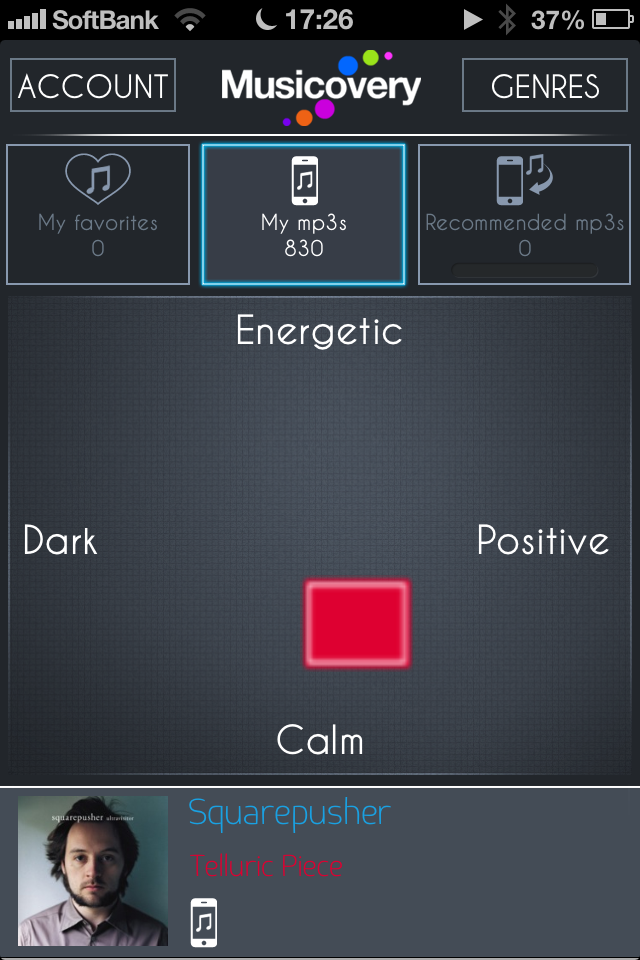
\includegraphics[width=5.866cm]{musicovery.png}
\caption{Musicoveryのインターフェース}
\label{musicovery_interface}
\end{center}
\end{figure}

\subsection{研究課題として時刻に注目した背景}
\subsubsection{研究の背景}
ジャンル名や、アーティスト名などの楽曲の音楽の情報自体にアクセスするのではなく、
どんな時刻にどんな楽曲が再生されたか、
どんな場所でどんな楽曲が再生されたのか、
どんな気分でどんな楽曲が再生されたのかなど、
楽曲が再生される状況と楽曲の関係性から、
楽曲を推薦することができるのではないかと考えた。
そこで、音楽再生時のユーザー自身の状況から、
音楽を推薦するために、いくつかの要素を抽出して、
予備的な音楽再生ソフトを自作して、
自分で使ってみたり、
プレゼンやデモを通して第三者からもフィードバックをもらうことで、
ユーザーの音楽を再生するときには、
どんな情報が、音楽の再生に影響をもたらしているのかを探ろうとした。
そして、いくつかの実験を踏まえて、
最終的に時刻に着目し、
本研究に至ったその背景をここで説明したい。
以下に自分が作ったアプリケーションを紹介する。
\begin{enumerate}
\item
場所の情報に注目して作ったもの

\subsubsection{Music Earth}

\begin{figure}[h]
\begin{center}
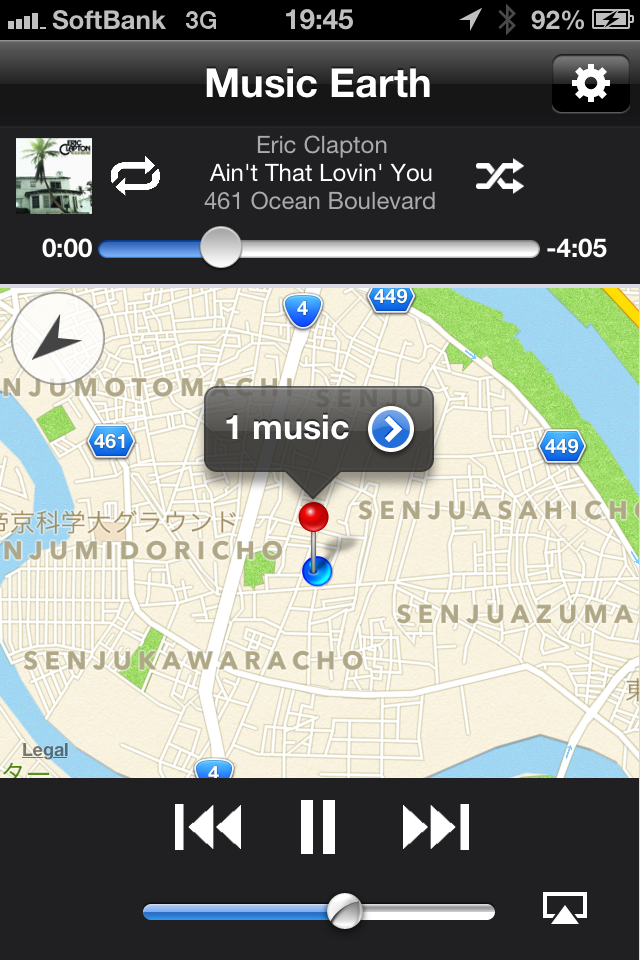
\includegraphics[width=5.866cm]{musicEarth.png}
\caption{Music Earthのインターフェース}
\label{musicEarth_interface}
\end{center}
\end{figure}

GPSを利用して音楽の履歴情報を地図にプロットしていくことで、地図全体が音楽のプレイリストとなり、
再生時の位置情報によって、以前その場所周辺で再生された楽曲の中からその場所に近ければ近いほど高確率で推薦される音楽再生アプリケーション。
iPhone用のアプリケーションで、iPhoneの音楽ライブラリと連携している。
音楽を聴いたら、地図上に聴いた位置情報と、聴いた楽曲を記録する。
地図から以前その場所で聴いた音楽を選択して聴くこともできる。
\subsubsection{Place Melody}

地図に聴きたい音楽を配置していき、自分がその場所に近づくと再生されるiPhone用アプリケーション。
選択しなければいけない音楽再生ではなく、場所から聞こえてくる音楽ということとをテーマに制作した。
電車に乗っていても音楽によって、目的地に到着したことを知ることができるなど、場所によって自分の音楽体験をデザインすることができる。

\begin{figure}[h]
\begin{center}
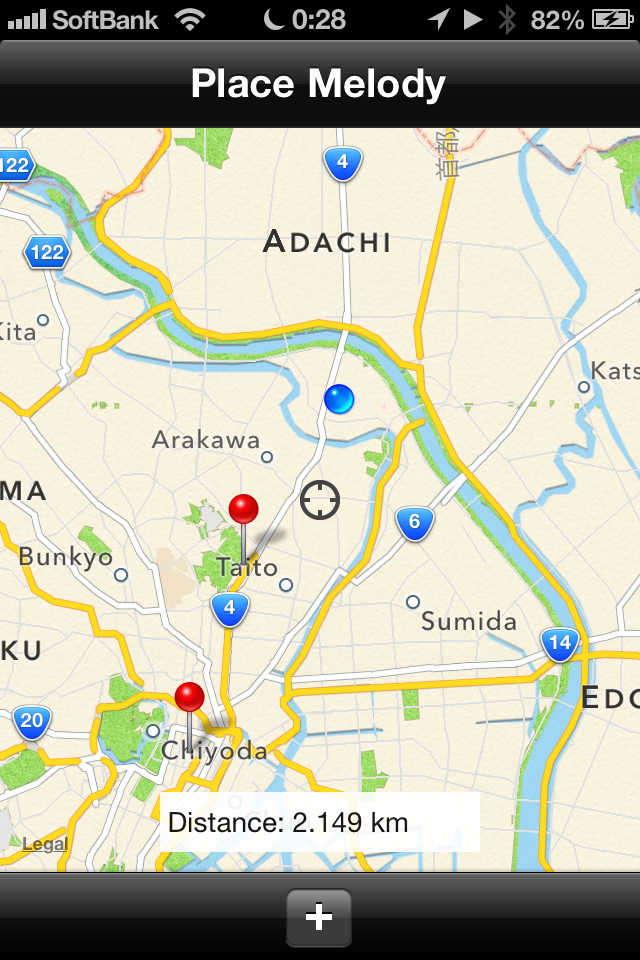
\includegraphics[width=5.866cm]{placeMelody.png}
\caption{Place Melodyのインターフェース}
\label{placeMelody_interface}
\end{center}
\end{figure}


\item
音楽再生における時刻とシーンに注目してつくったもの

\subsection{OtO}
ユーザーが楽曲を聴いた時間を学習し、図\ref{OtO_playlist}に示すように、
曜日毎に0時から24時までを1時間区切りでプレイリストをつくる。
ユーザーが自動的に再生したいときは、シーンを選択して、
その時刻にそのシーンで以前聴いた音楽のなかからランダムで楽曲が選ばれて再生される。
Mac用のアプリケーションでiTunesと連携している。

\begin{figure}[h]
\begin{center}
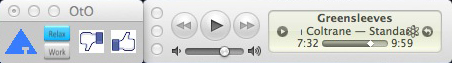
\includegraphics[width=5.866cm]{OtO_imageView.jpg}
\caption{OtOのインターフェース}
\label{OtO_interface}
\end{center}
\end{figure}

\begin{figure}[h]
\begin{center}
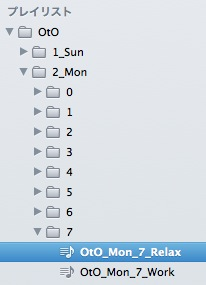
\includegraphics[width=5.866cm]{OtO_playList.jpg}
\caption{OtOのプレイリスト}
\label{OtO_playlist}
\end{center}
\end{figure}


音楽を再生する際にシーンを選択してもらうことによりシーンにあった音楽を推薦する方式。
\end{enumerate}

以上の音楽アプリケーションのプロトタイプを体験してみて、
場所については、場所によって異なる音楽を聴いていることもあったが、
それは、場所自体に直接的な意味合いがあるというよりも、その時刻にその場所にいることが多いという、間接的な関係であり、時刻に比べて相関が薄かった。
例えば、移動中であったときは、状況は移動中であるだけなのにもかかわらず、移動している場所にちりばめられるといったことが起こった。
また、同じ場所であっても、休憩中や、作業中などの様々なシーンに応じて音楽を選んでいる場合でも、一元化されてしまうといった問題点もあった。
シーンを選ぶものは、ユーザー自身で``リラックス中''や``作業中''といった、音楽を再生するシーンを選択してもらうので、実際にはプレイリストを自作する行為に似ており、
音楽推薦機能としてのメリットが小さくなってしまった。
また、楽曲をシーンに分類するためには、ユーザーが特定のシーンを選択する行為の膨大な学習期間を要することも問題だった。
時刻に関しては、場所、シーンの両方ともに関係しており、
音楽を再生する際に、ユーザーの状況を説明するのに、最も基本的な要素であり、直接的だったため、
時刻の情報がユーザーの音楽再生における状況において、もっとも重要だと推測した。
%そして、実際に、時刻がユーザーの音楽再生にどのような影響を与えるのかを明らかにすべく、
%音楽再生と時刻の関係についての研究をすることに至った。

%\subsection{既知の障害}
%人によって、生活が不規則な人もいると容易に推測できるために、時間によって、傾向が出ないことも考えられる。
%必ずしも時間と音楽の再生に相関がある人ばかりではないことも留意しつつ、調べる必要がある。
%そのため、音楽の再生時刻だけでなく、普段の生活がどのようになっているのかを直接知る必要がある。
%また、iTunesの履歴からは、
%シャッフル機能を使用して再生されたのか、
%ユーザーの操作によって選択されて再生されたのかを、
%区別して分析することは難しいので、
%再生履歴を一元的にユーザーによる積極的な選択としてみなすことが出来ない場合も注意する必要がある。
%また、ソフトの仕様により、履歴情報が全て記録されていない場合があり、
%今回使用したiTunesでは、ひとつの楽曲に対して、最後に再生した時刻だけしか記録されていない。
%全てを保存するアプリケーションを自作することも可能だったが、
%その場合、従来の音楽再生スタイル自体を大きく変化させてしまうことで、
%従来の履歴情報を取得することが困難になると考えたため、
%この点においては妥協してiTuensを使用することにした。
%音楽再生のスタイルがユーザーインターフェースに依存してしまう可能性があるが、
%iTunesは音楽を選択する自由度が高いので、iTunes自体が音楽の聴き方を制限することがないと考えた。
%
%また、ジャンル名を取得できていない楽曲もあり、
%またユーザーが手動で設定しなくても、iTunesが自動的につけるために、
%ユーザーが考える楽曲のジャンルと、iTunesが付けたジャンルとが必ずしも合致するとも限らない。

\subsection{研究動機}
%ユーザーの状況を推測することは容易ではない。
%また、ユーザーの状況をユーザー自身が入力することも容易ではない。
%そのため、ユーザーの状況を推測することが可能であり、ユーザーの入力負担が小さいものが求められる。
%いくつかのプロトタイプアプリケーションを試したことから、時間情報が有効であると判断した。
%時刻情報であれば、特別なセンサーも不要なためどのような機器に対しても、
%時刻情報による、音楽推薦機能を組み込むことができる。

音楽推薦機能に時刻情報が有用かどうかを調べるために、
時刻と音楽がどのように関係しているのか、関係していないかを明らかにする。
以前は例えば自宅で夜、音楽鑑賞するといった決まった状況で聴いていたため、
音楽を再生する外的な状況に別段の変化はなかった。
しかし、モバイルプレイヤーにおける音楽の再生は、場所や時間を選ばない。
そのため、モバイルプレイヤーの使用者は様々な場所や時間において、自分で音楽を再生する音楽を選択する必要が出てきた。
すなわち、音楽推薦システムが推薦する相手であるユーザーの状況が多様になってきたことを意味する。

ユーザーは、状況が変化すると、音楽を再生する動機や気分などに差が出ると推測し、
外的な状況の変化に対して、音楽の再生がどのように変化しているのかを、特に時間情報に注目して調べることにした。
時刻情報によって音楽再生が動的に変化しているのであれば、音楽推薦システムも同様に時刻情報によって動的に変化するべきであると考えた。

\subsection{方針}
本研究では特に時刻に注目して、時刻によって音楽の聴き方がどのように変化するのかを調べた。
時刻に注目した理由は以下の通りである。
\begin{itemize}
\item
規則的、周期的である。
ほとんどの場合、朝は自宅から始まり、夜は再び、自宅にもどる。
その時間も人によってではあるが、パターン化されていると考えられる。
そのため、時刻だけからもある程度、人の営みを推測することができそうだと推測できた。
\item
音楽と相関がありそうである。
現状で、モーニングコンサートや、オールナイトコンサートなど、時刻を表す言葉を冠したものや、
ジャズや、ダンスのクラブは夜行われていることが多く、時刻と音楽のシーンが組み合わさることは見慣れている。
そのため音楽には時刻的な要素が存在していると予測できた。
\end{itemize}

%\subsection{期待される成果}
%今後の展望?
%場所情報と組み合わせることで状況をより正確に推測したり、
%シーンを時間から推測したりといった拡張性に期待したいと考えた。
%ジャンルによる推薦方式と組み合わせることで、ユーザーの聴きたい音楽を再生する精度が高まることを期待する。
%例えば、朝の時間はクラシックを中心に聴くことをを好み、夜には、ジャズを中心に聴く人がいたとすると、
%ジャンルによる音楽推薦システムでは、ジャズとクラシックを交互に再生するリコメンドとなってしまうので、
%ユーザーの聴きたい音楽を推薦する精度は小さくなる。


\section{分析手順}
\subsection{被験者について}
本実験の被験者は普段iTunesを利用して音楽を聴く20代の20名の大学生ある。
被験者は普段から、iTunesと同期しているモバイルプレイヤー(iPod, iPhoneなどのアップル社製の機器)を利用している。

被験者をiTunesを利用している人に限定したのは以下の理由である。
\begin{itemize}
\item
スマートフォンに関しては、インターネット白書2011によると、
所有しているスマートフォンはiPhoneが47.7\%と最も高いこともあり、
多くの人がiTunesをモバイルでも利用しているため、被験者を集めやすいということ。
\item
iTunesはユーザーの音楽再生の履歴情報を記録している。iTunesはiTunes内で管理している全ての楽曲について、 最後に再生された時刻を記録している。
\item
履歴データには、
ラップトップ型コンピュータや、
デスクトップ型コンピュータなどを利用して、
自宅でiTunesを利用して音楽を再生した情報と、
携帯音楽プレイヤーまたは、音楽再生機能を有した携帯電話を利用して、
外でiTunesを利用して音楽を再生した情報が、
どちらも1つの履歴ファイルに統合されている。
\item
楽曲のジャンル名はユーザーがタグ付けしなくても、iTunesによって自動的にタグ付けされる。
\end{itemize}

\subsection{分析手法について}
被験者がどんな時刻にどんな音楽を聴いているのかを被験者の履歴データから調べる。
また、以下の理由により、被験者に、普段の生活と音楽再生についてのアンケートを書いてもらった。

%アンケートのサンプル画像
\begin{figure}[htbp]
\begin{center}
\fbox{							
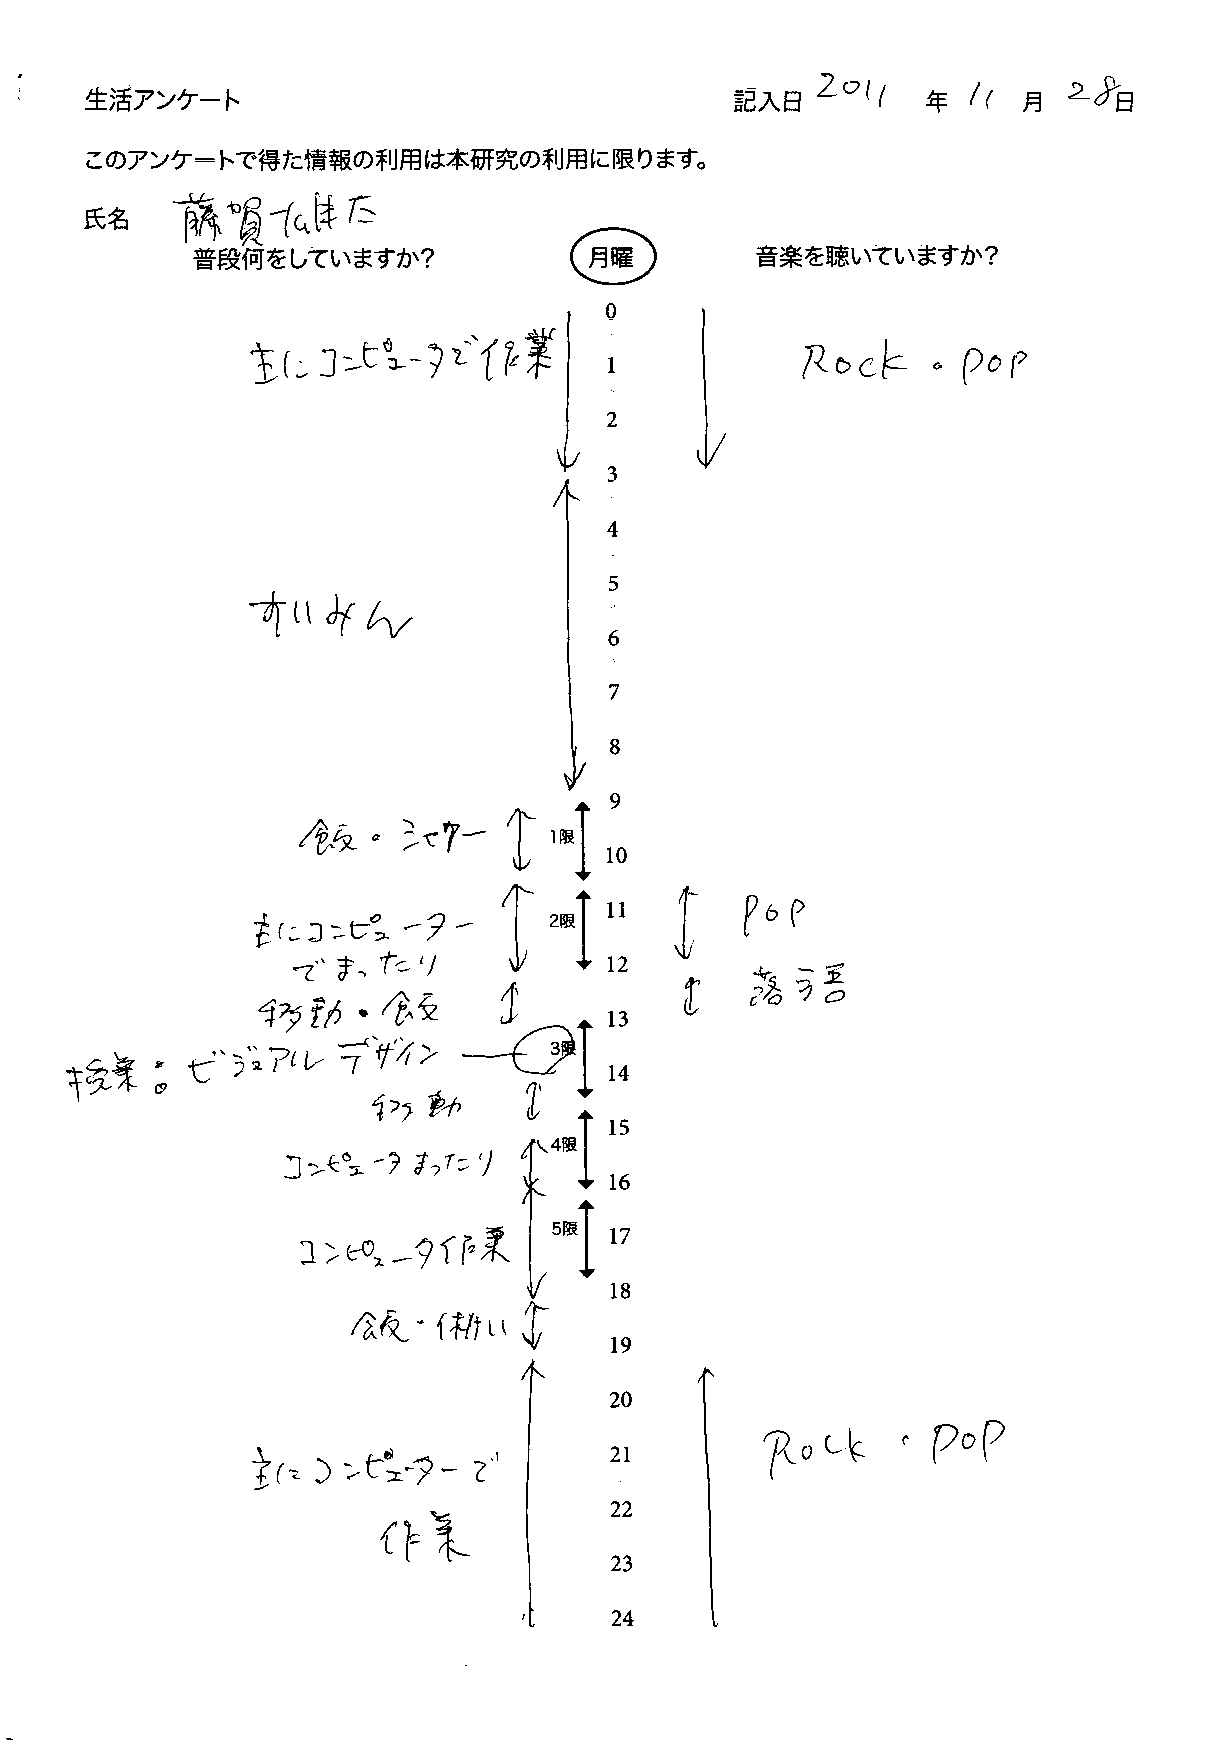
\includegraphics[width=7cm]{musicLifeSheet_sample.pdf}
}
\caption{アンケートシートのサンプル}
\end{center}
\label{sheet_sample}
\end{figure}

\begin{itemize}

\item
本研究の中での曜日は、被験者によって定義が異なる。
通常であれば、1つの曜日の範囲は0時0分0秒から23時59分59秒であるが、
本研究では、音楽を聞いて時間帯を睡眠時間と推測できるほか、
アンケート用紙にて普段の睡眠時間を曜日ごとに書いてもらい、
個人毎に起きている時間帯を曜日の範囲として定義した。
そのため、曜日によっては24時間よりも長くなったり、短くなったりしている。
また、0時0分からではなく、
起床したと思われる時間を曜日の開始、24時0分ではなく、
就寝したと思われる時間を曜日の終わりと定義した。

履歴データから生成された音楽再生履歴を表すグラフからは、
音楽を聴いていない深夜からの時間を睡眠時間ではないかと予想できるため、
ある程度の曜日の切れ目を推測できるが、
4時や5時などに音楽が再生されている場合、
深夜に聴いたのか、
早朝に聴いたのか判別がつかない。
そこで、アンケートに書かれた睡眠時間を参考にしてどちらなのかを決定する。
\item
シャッフル機能を使用して再生されたかどうかは、iTunesは履歴として記録しないため、
ユーザーが自分で意図的に聴きたい曲を選択したのか、自動的にiTunesによって再生されたのかどうかは履歴ファイルからは判別がつかないため、アンケートに、シャッフルを使用したかどうかを書いてもらった。
\item
何をしている時にその音楽が再生されたのかはiTunesの履歴データにはない情報である。
そのため、ユーザーの音楽を再生する状況が時刻によって変化しているのかどうかを調べるために
アンケートに普段の生活を書いてもらった。
\end{itemize}


被験者に渡したアンケートシートは、0時から24時までを30分刻みで目盛りを付けたもので、
普段の生活と、普段の音楽聴取を記入してもらうもので、月曜日から日曜日までの合計7枚のものである。
不規則な生活、気まぐれな音楽再生など、毎週規則正しくない部分は備考として記入してもらう。
普段聴く音楽の項目に関しては、iTunesを利用した情報のみを書いてもらった。
また、聴く音楽の内容が決まっている場合は、ジャンル名やアーティスト名などを書いてもらった。
普段の生活を各項目については、30分刻みを目安に書いてもらった。
図\ref{sheet_sample}に示すように、
用紙の中心に時間軸が書かれており、
その時間軸の左側に普段の生活について、
右側に普段の音楽再生についてを書いてもらうため、
左右を見比べることで、どんなことをしているときに、
どんな音楽を聴いているのかがわかるようになっている。

履歴データから得られる、被験者の音楽再生履歴と、アンケートを見比べることで、
再生時の状況と音楽選択の関係性を明らかにする。

また、被験者は学生だったため、年度によって授業が変化し、音楽再生の時刻に影響があると考えたため、
2012年度、すなわち2012年4月1日0時0分0秒から2012年12月10日までの履歴データに限定した。
\subsection{分析の流れ}
実験は以下の手順で進めた。

\begin{enumerate}
\item
被験者20名(iTunesをいつも利用して音楽を聴いている大学生)からiTunesの履歴ファイル(xmlファイル)をメール添付でもらう。
\item
被験者に図\ref{sheet_sample}に示すように自分の生活を曜日毎にアンケートシートに書いてもらう。
\item
履歴ファイルから、以下の情報を読み取って、
どの曜日の、
どの時刻に、
何回聴いたのかを示すグラフをつくる。
なお、iTunesに記録されている履歴情報は最後に聴いた時刻だけなので、
複数回聴かれている場合でも、最後に聴いた時刻だけを分析に使用する。
\begin{itemize}
\item
楽曲のジャンル
\item
最後に聴いた日付・時刻
%\item
%再生回数
\end{itemize}

%\begin{figure}
%\begin{center}
%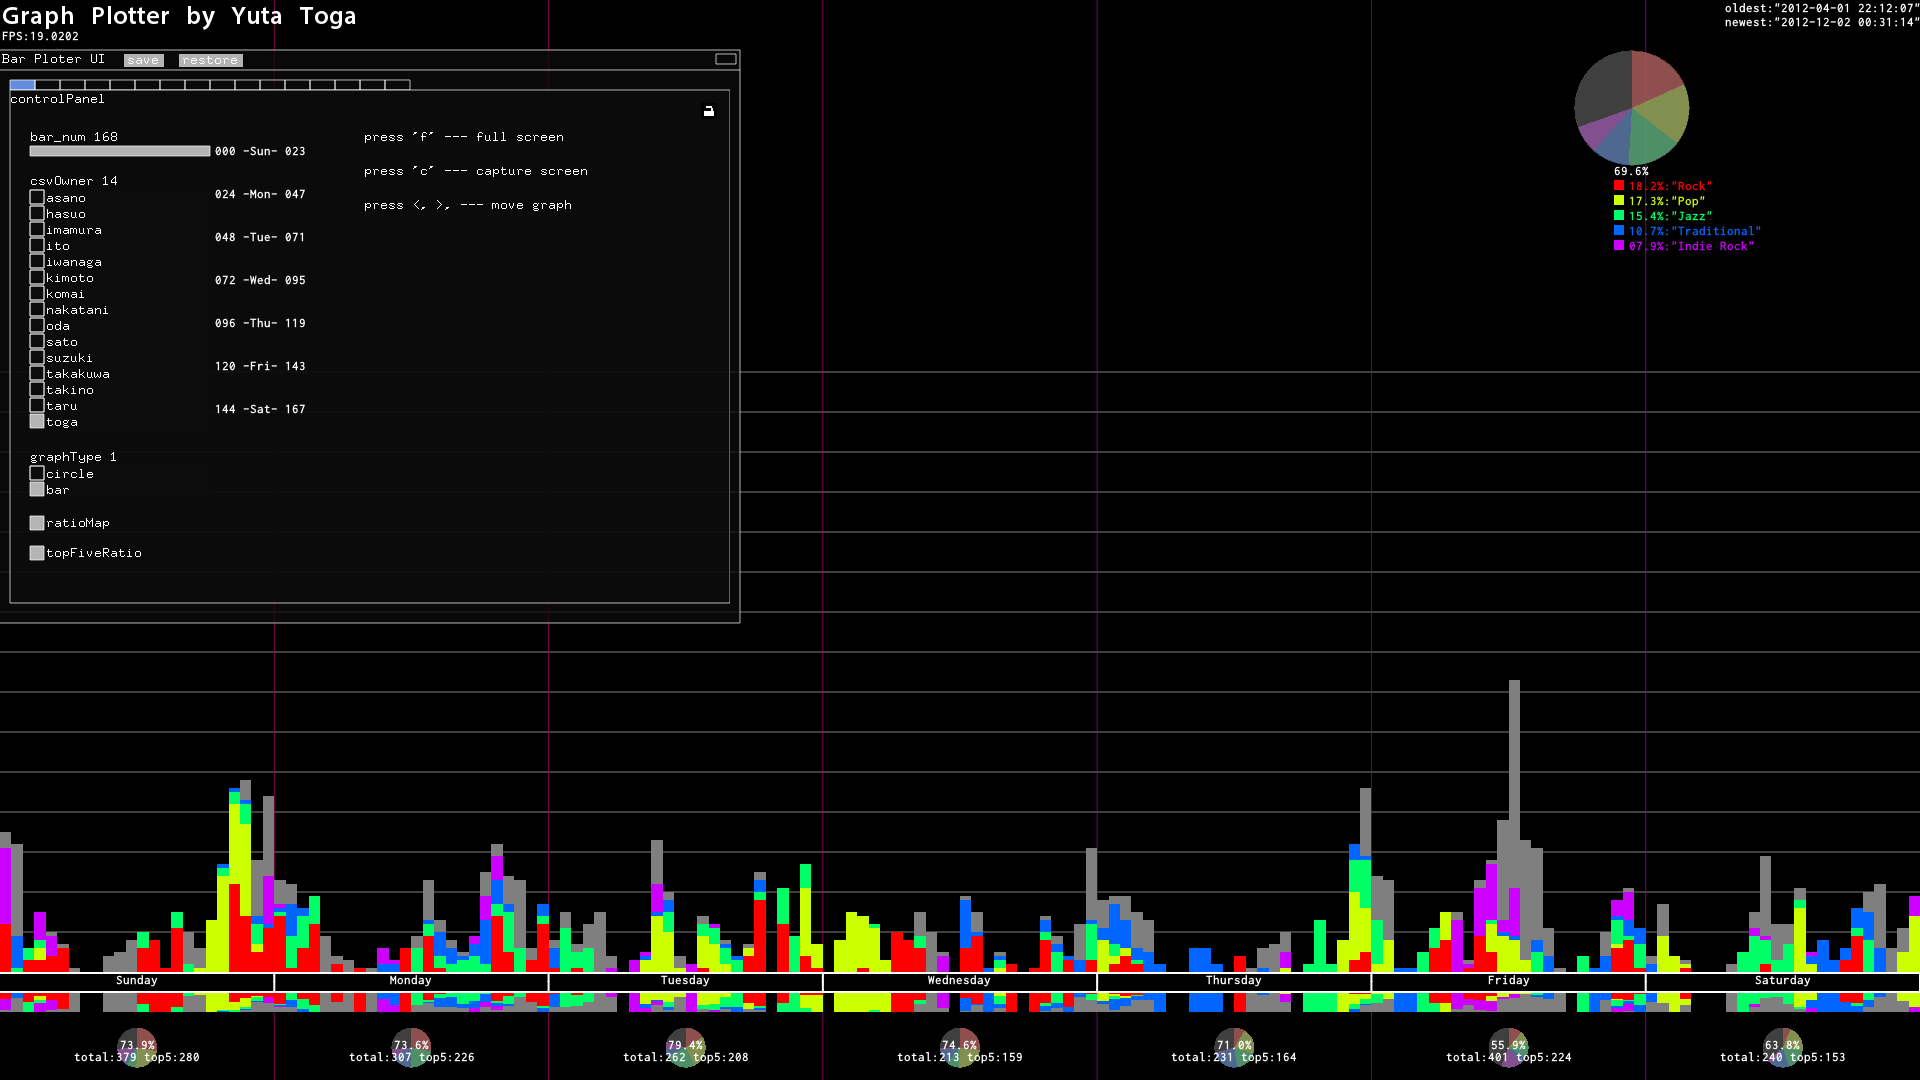
\includegraphics[width=7cm]{graph_sample.png}
%\caption{分析結果のグラフの一例}
%\end{center}
%\end{figure}

\item
被験者のアンケートシートで得た音楽再生の情報と、
被験者の音楽再生の履歴データから生成したグラフを比較しながら分析を行う。
\item
被験者のアンケートで得た情報によると音楽を聴いてない時間であるにもかかわらず、
履歴データからは、音楽が多く聴かれているといったように、
アンケートで記載されたことと、
履歴データから読み取られる内容が異なる場合には、
違いについてインタビューを行い、
なぜ違ったのかを明らかにする。
\end{enumerate}

\section{結果}
寝ている間に聴く、または、生活が極端に不規則という人以外の多数は、
寝ている時間を音楽の履歴データによっておおよそ推測できた。
また、必ず聴いていない時間が存在することがあり、その時間はバイトや授業などが毎週あることが多かった。
また、毎週決まって聴く時間があると、その場所だけ、再生回数が群を抜いて大きくなる。
そのため、数回しか聴いてない情報を省いて分析をすると、
定期的に音楽を聴く時間帯が見えてくる。

また、人によっては金曜の夜だけ多く聴いているというような、曜日による偏りが見られた。
個人単位で大きくことまる音楽の聴き方をしており、被験者の数もパターン化するほど多くなかったため、
具体的に特徴的な人の例を以下に示すことにする。

\subsection{規則的な人}
規則的な人の音楽再生を表すグラフを、図\ref{sample_regular}に示す。
グラフの横軸は時間軸を表しており、1時間毎に棒グラフを描いてある。
すなわち、
一番左の棒グラフは日曜日の0時0分0秒から0時59分59秒までの再生回数を示しており、
一番左の棒グラフの右隣の棒グラフは、日曜日の1時0分0秒から1時59分59秒までの再生回数を示しており、
一番右の棒グラフは、土曜日の23時0分0秒から、23時59分59秒までの再生回数を示している。

グラフの縦軸は再生回数を表している。
棒グラフは累積グラフになっており、下から、ユーザーが再生した楽曲のジャンルの中で最も多い順から色分けされている。
図\ref{sample_regular}では、6色に色分けされているが、下から、
最も聴かれたジャンル、
2番目に聴かれたジャンル、
3番目に聴かれたジャンル、
4番目に聴かれたジャンル、
5番目に聴かれたジャンル、
その他のジャンルの
それぞれの再生回数を表している。

\ref{sample_regular}のグラフに示すように時間に決まった時間に音楽を聴いている。
規則的に音楽を聴く人は、アンケートシートで調べた普段の生活も、非常に規則正しい生活をしている。
特に、寝る時間や、起きる時間、外出する時間、帰宅する時間が規則正しいので、
聴いていない時間はほとんどきいておらず、聴いている時間はかなり聴いているため、凹凸の激しいグラフとなっているのがわかる。
寝ている時間が音楽を聴いていない時間帯から推測することができた。

\begin{figure}[h]
\begin{center}
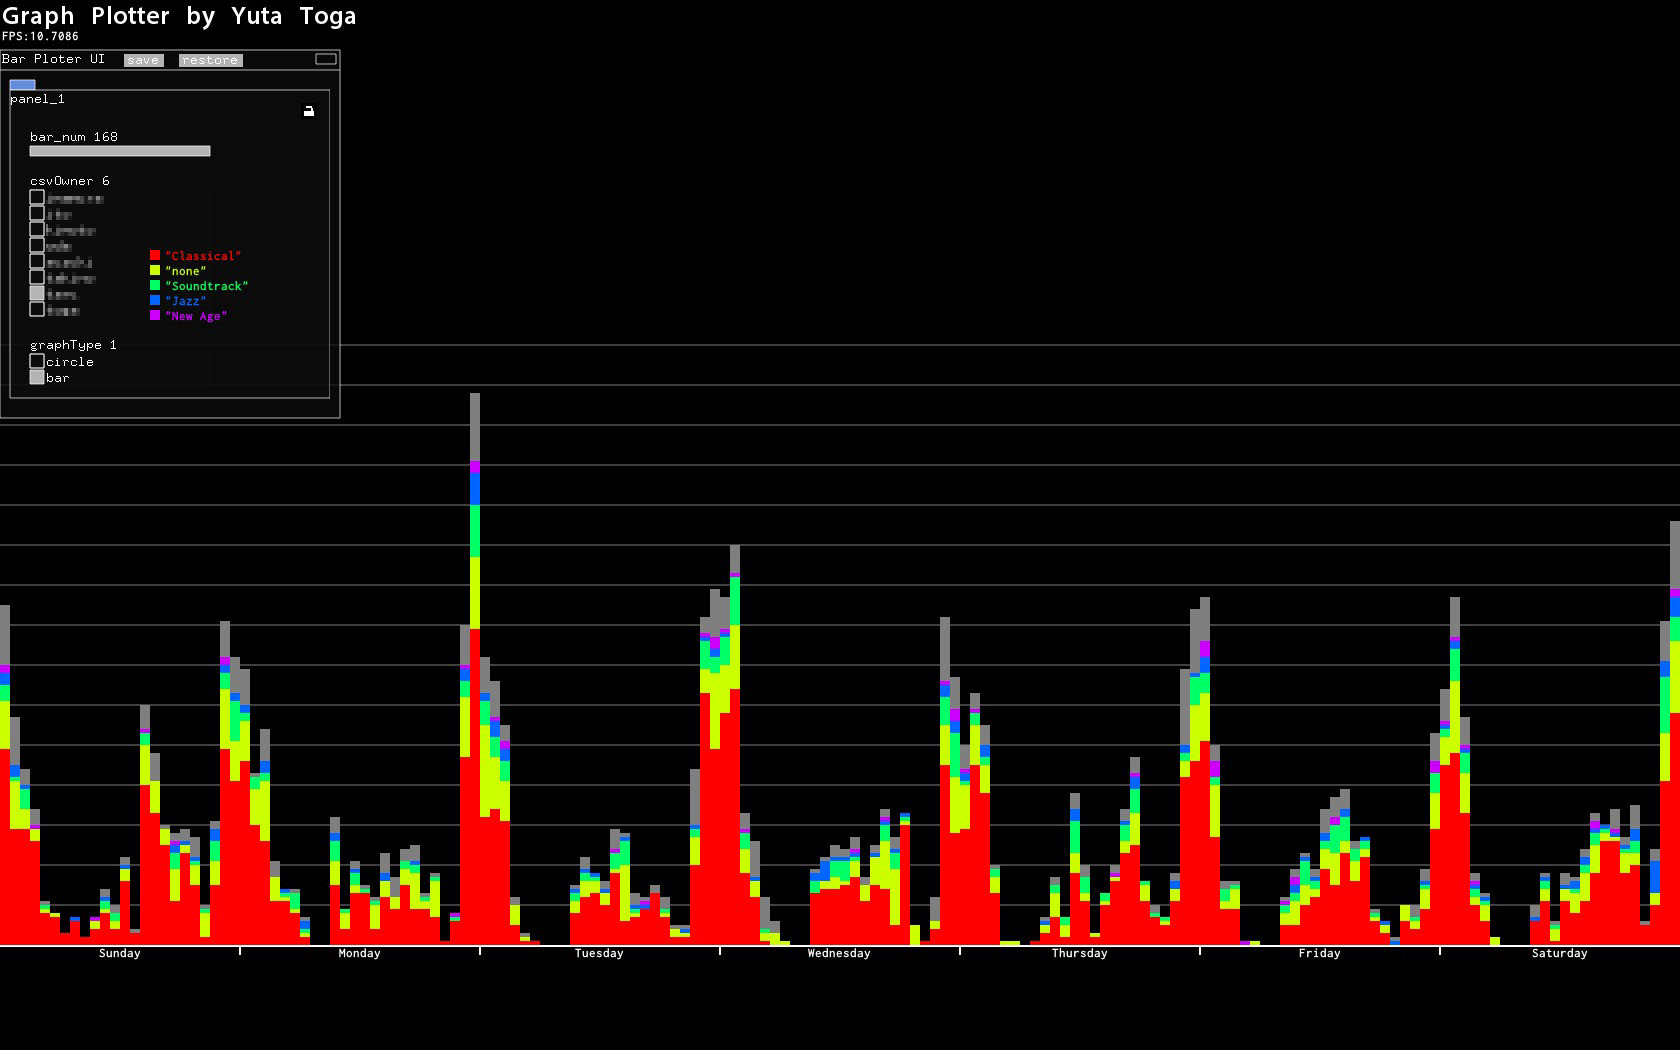
\includegraphics[width=14cm]{sample_regular.jpg}
\caption{規則的な人の例}
\label{sample_regular}
\end{center}
\end{figure}

\subsection{不規則な人}
不規則な人は、図\ref{sample_irregular}のグラフに示すように規則的な音楽再生は見られない。
音楽によって、睡眠時間を推測することが困難で、どこに曜日の切れ目があるのか曖昧であった。
深夜アルバイトをしている学生が、翌日に複数回に分けて数時間睡眠するといったことも見られ、
7つの曜日それぞれの時刻を定義することが難しい例もあった。

\begin{figure}[h]
\begin{center}
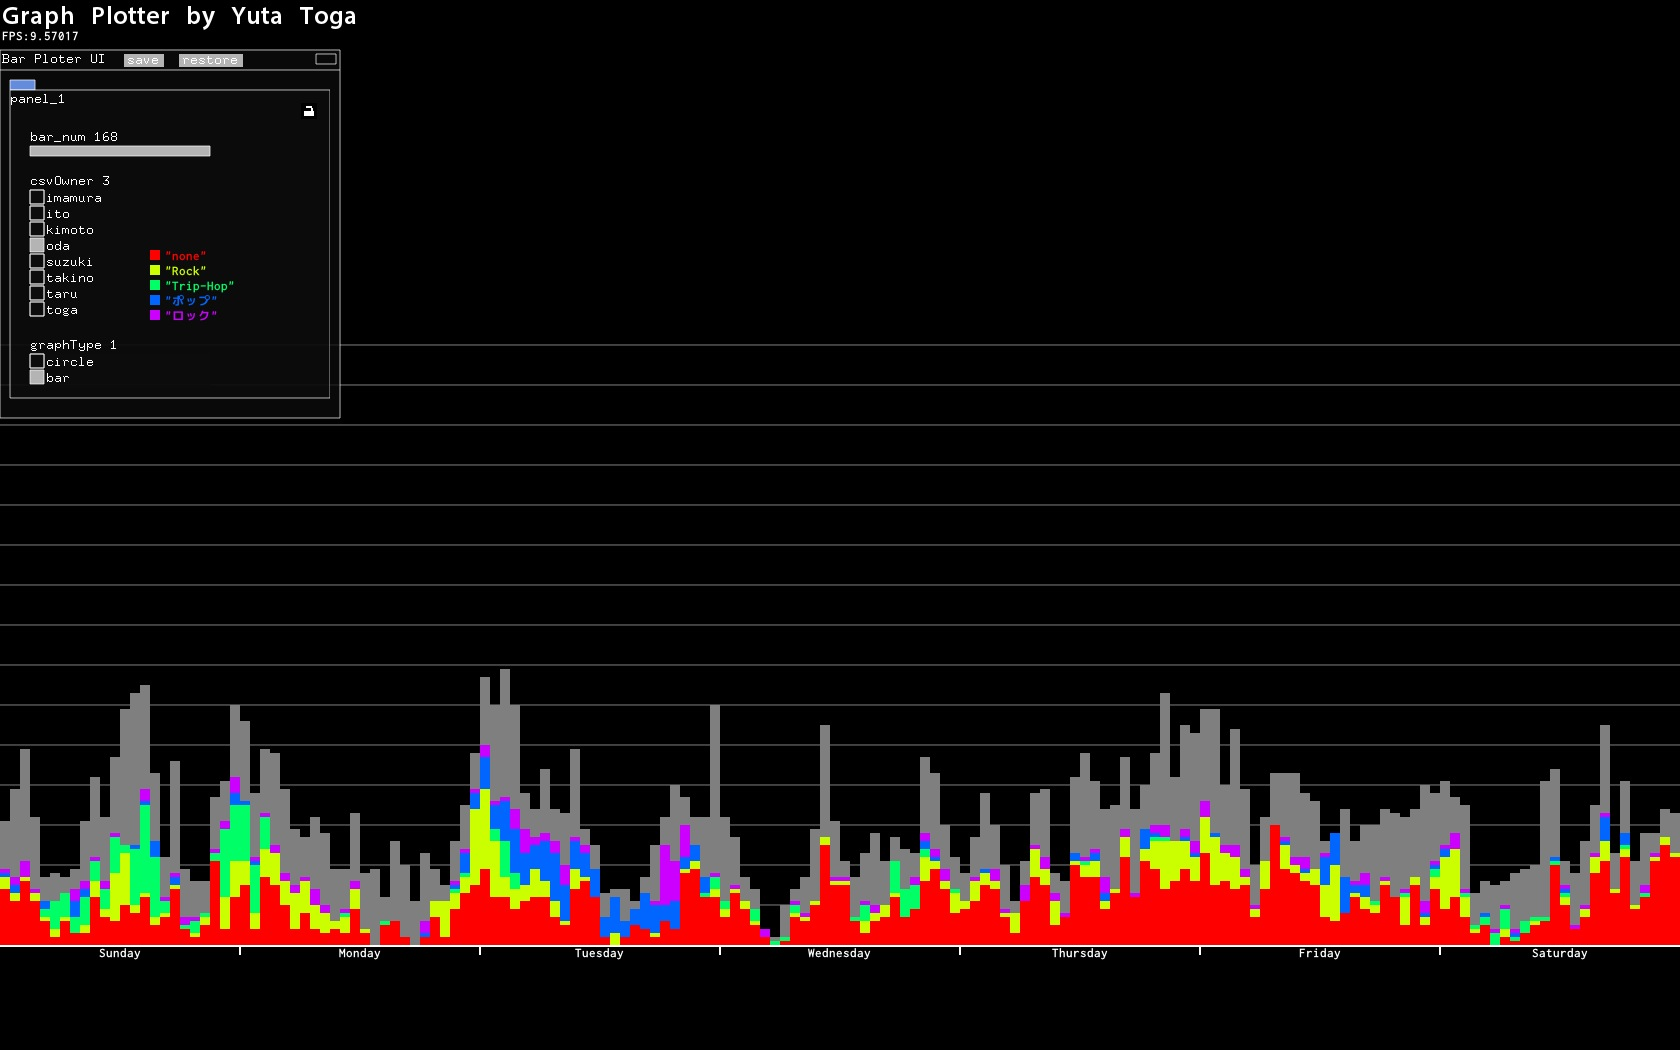
\includegraphics[width=14cm]{sample_irregular.jpg}
\caption{不規則な人の例}
\label{sample_irregular}
\end{center}
\end{figure}

\subsection{音楽ジャンルの分布が一定な人}
図\ref{genreMap_regular}は、音楽ジャンルの内訳を示すグラフである。
これは、音楽再生の回数ではなく、
音楽再生のジャンルの内訳の比率を高さで表したものである。
グラフの横軸は時間軸を表しており、1時間毎に棒グラフを描いてある。
一番左の棒グラフは日曜日の0時0分0秒から0時59分59秒までのジャンルの内訳を示しており、
一番左の棒グラフの右隣の棒グラフは、日曜日の1時0分0秒から1時59分59秒までのジャンルの内訳を示しており、
一番右の棒グラフは、土曜日の23時0分0秒から、23時59分59秒までのジャンルの内訳を示している。

縦軸がジャンルの内訳を示してある。
図\ref{genreMap_regular}では、6色に色分けされているが、上から、
最も聴かれたジャンル、
2番目に聴かれたジャンル、
3番目に聴かれたジャンル、
4番目に聴かれたジャンル、
5番目に聴かれたジャンル、
その他のジャンルの
それぞれの比率を表している。

なお、再生されていない時間は、棒グラフを描いていない。

図\ref{genreMap_regular}が示すように、
音楽再生のジャンルの内訳調べたとき、時刻や曜日が変化してもジャンルの内訳は一定な人がいた。
これは、シャッフル機能を利用して再生しているために、
iTunesに入っている音楽ライブラリのジャンル構成がそのまま音楽の再生の分布になっていると考えられる。
実際に、アンケートと併せて分析すると、
こういった音楽再生のジャンルの分布をとる人はシャッフル再生を好んで利用している傾向があることがわかった。

\begin{figure}[h]
\begin{center}
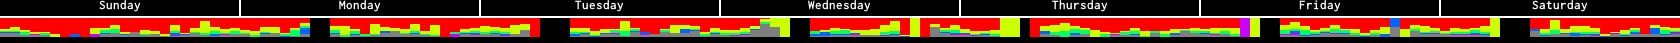
\includegraphics[width=14cm,height=2cm]{genreMap_regular.jpg}
\caption{音楽ジャンルの分布が一定な人の例}
\label{genreMap_regular}
\end{center}
\end{figure}

\subsection{音楽ジャンルの分布むらがある人}
図\ref{genreMap_irregular}に示すように、
音楽ジャンルの分布にむらがある人がいた。
図\ref{genreMap_irregular}と\ref{genreMap_regular}を見比べると、
時刻や、曜日によってジャンルの内訳が変化していることが読み取れる。
この傾向は、音楽再生において、以下のような人にこの分布をとる傾向があった。
\begin{itemize}
\item
シャッフル機能を使用せずに、自分で逐一選択して音楽を再生する。
\item
音楽を聴く際に、音楽を聴く以外の作業、
例えば、本を読みながら音楽を聴く、
電子メールを書きながら音楽を聴くといった``ながら聴き''ではなく、
音楽を聴くことに集中して音楽を再生する。
\end{itemize}
また、アンケートには時間によって音楽の内容を変えていると書いていない人の中にも、
履歴データの分析によると、曜日によって再生しているジャンルの内訳が異なるといったことがあった。


\begin{figure}[h]
\begin{center}
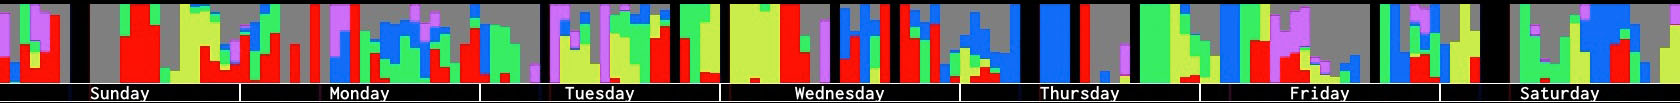
\includegraphics[width=14cm, height = 2cm]{genreMap_irregular.jpg}
\caption{音楽ジャンルの分布にむらがある人の例}
\label{genreMap_irregular}
\end{center}
\end{figure}

\subsection{聴いているジャンルの偏りが大きい人}

%\begin{figure}[h]
%\begin{center}
%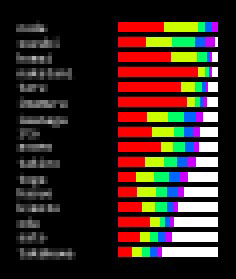
\includegraphics[width=7cm]{sortedOther.jpg}
%\caption{iTunesのなかのライブラリーのジャンルの内訳全員分}
%\label{sortedOther}
%\end{center}
%\end{figure}

再生された音楽のジャンルの内訳の中で、上位のジャンルが占める比率を出した結果、
図\ref{topFive_heavy}のようにジャンルの上位によって、ほぼすべての曜日、ほぼすべての時間で、ほとんどを占めている場合がある。
図\ref{topFive_heavy}の右上の円グラフは、音楽ライブラリー全体のジャンルの内訳である。


\begin{figure}[h]
\begin{center}
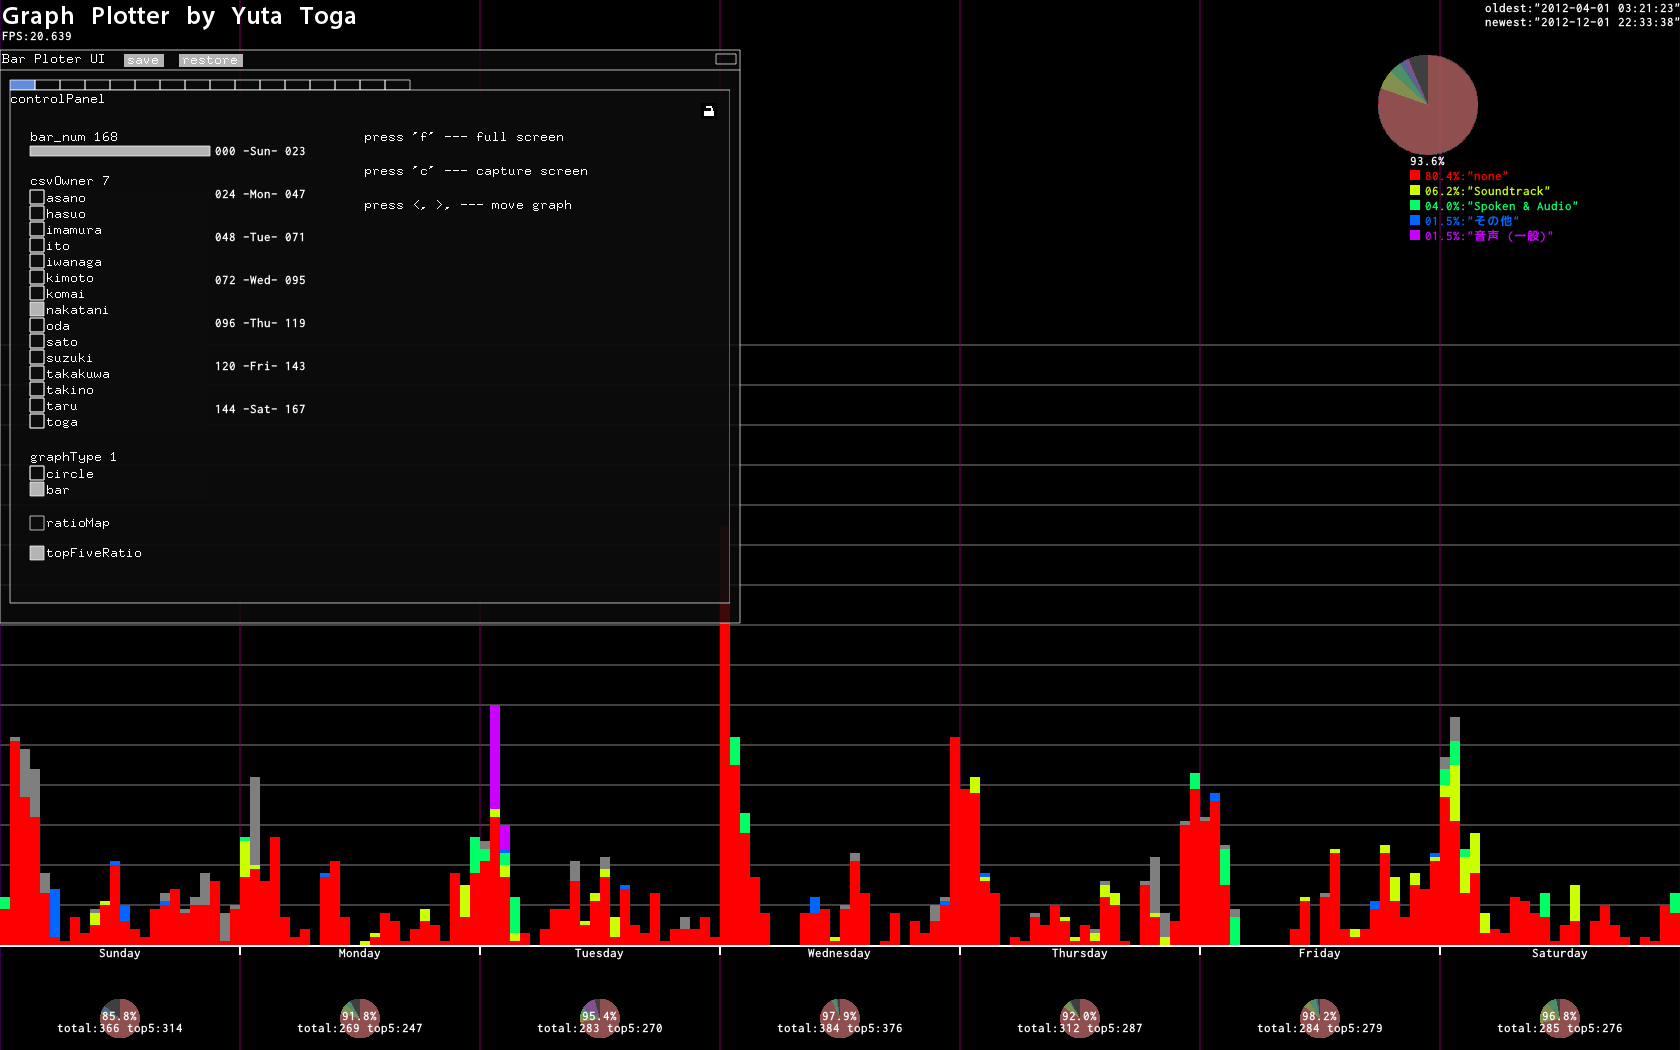
\includegraphics[width=14cm]{topFive_heavy.png}
\caption{上位のジャンルによって多くを占めている人のグラフの例}
\label{topFive_heavy}
\end{center}
\end{figure}

\subsection{多くのジャンルを偏りなく聴いている人}
再生された音楽のジャンルの内訳の中で、上位のジャンルが占める比率を出した結果、
図\ref{topFive_light}のようにジャンルの上位が占める割合が小さい場合がある。
図\ref{topFive_light}の右上に示す円グラフは、音楽ライブラリー全体のジャンルの内訳である。
実際に、この傾向を持つ人にジャンルについてインタビューをしたところ、
ジャズの次にアイドルグループのポップスが再生されるといった、
ジャンルを超えた順番で音楽が再生されても抵抗感がないばかりか、
その驚き自体を楽しんでいるという回答を得た。


\begin{figure}[h]
\begin{center}
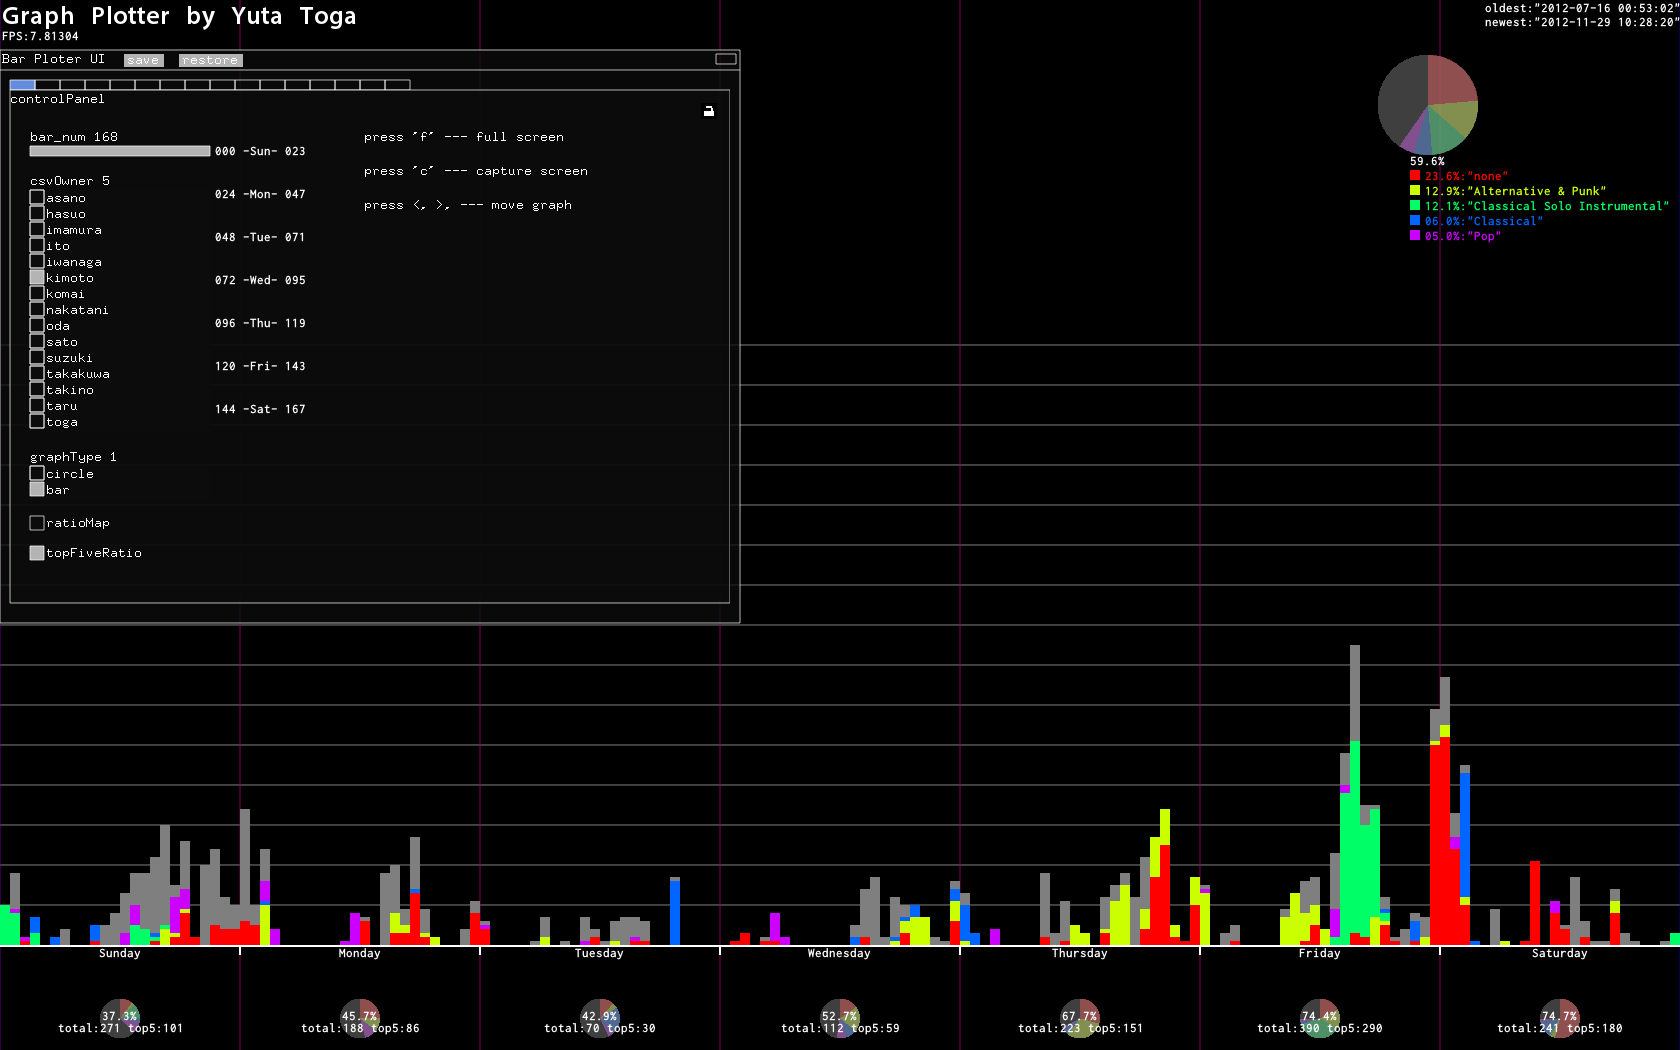
\includegraphics[width=14cm]{topFive_light.png}
\caption{上位のジャンルによって占められる割合が小さい人のグラフの例}
\label{topFive_light}
\end{center}
\end{figure}

\subsection{音楽をあまり聴かない人}
図\ref{lightListner}に示すようにあまり聞かない人は、
再生された楽曲のジャンルの内訳で、上位5つのジャンルによって占める比率が80%を超えることが多い。
また、音楽ライブラリ全体のジャンルの内訳と曜日毎に再生された音楽のジャンルの内訳の相関は小さい。

\begin{figure}[h]
\begin{center}
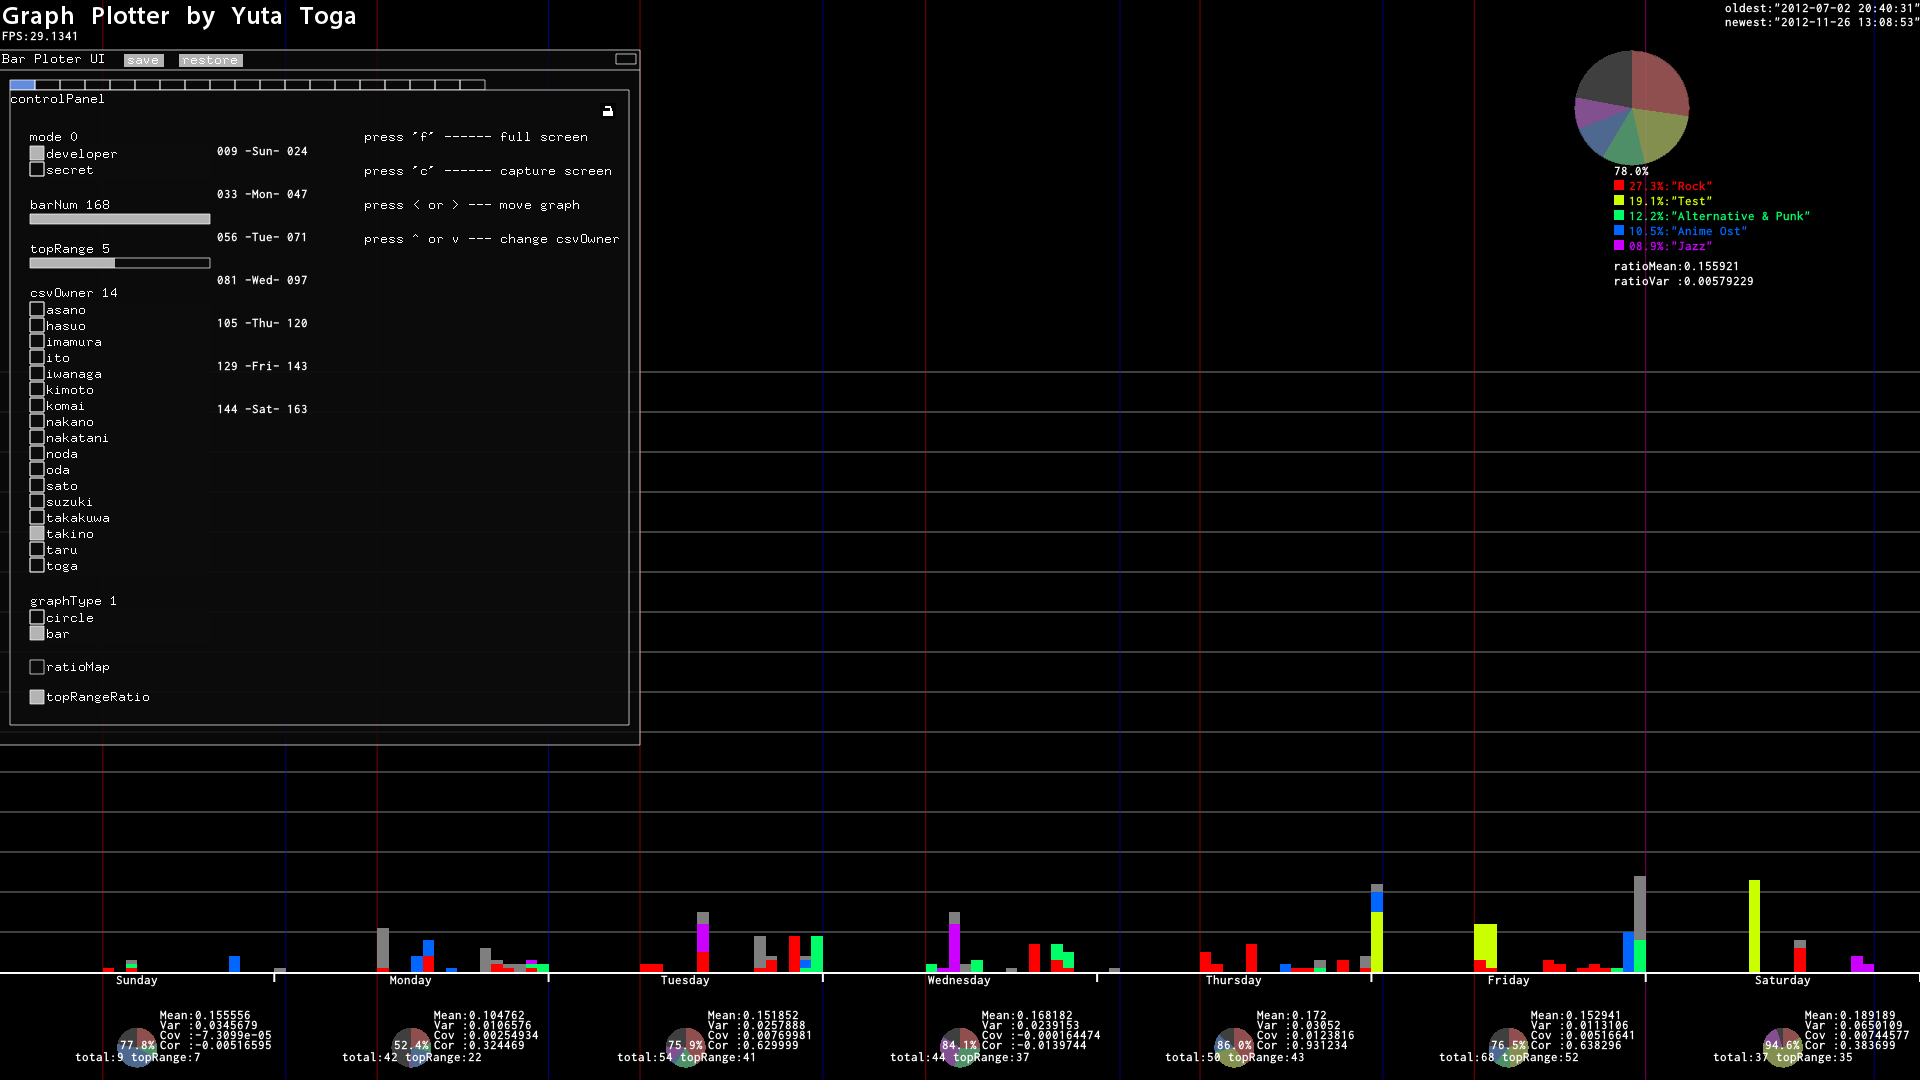
\includegraphics[width=14cm]{takino.png}
\caption{再生された音楽の内訳のうち、上位のジャンルによって占められる割合が小さい人のグラフの例}
\label{lightListner}
\end{center}
\end{figure}


\subsection{シャッフル機能を使う人のチェックマークの入った楽曲の例}
図\ref{checkedItemsGenreMap_shuffle}と図\ref{weekGenreMap_shuffle}を見比べると、
シャッフル機能を使う人の曜日毎に再生されたジャンルの内訳は
iTunes内のチェックマークの入っている楽曲全てのジャンルの内訳と相関が高いことがわかる。

これは、すなわち再生された音楽のジャンルの内訳の比率が、
ランダム再生で再々されるジャンル毎の再生確率とほとんど同じであるということを意味する。
このため、このユーザーは音楽をシャッフル機能を使用して再生しているのがわかる。

\begin{figure}[h]
\begin{center}
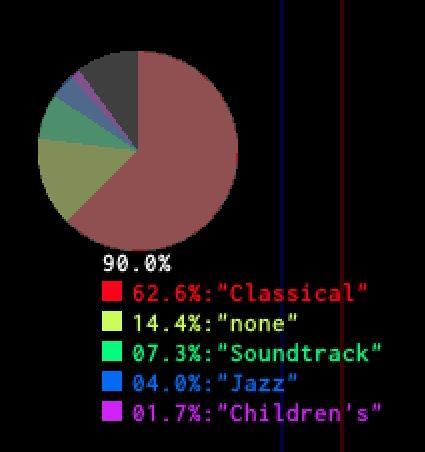
\includegraphics[width=7cm]{taru_checkedItemGenreRatio.jpg}
\caption{シャッフル機能を使う人のチェックマークの入った楽曲の例}
\label{checkedItemsGenreMap_shuffle}
\end{center}
\end{figure}

\begin{figure}[h]
\begin{center}
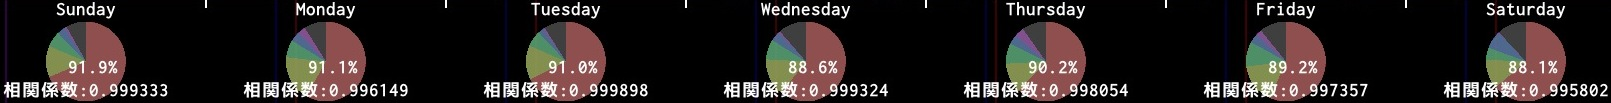
\includegraphics[width=14cm, height = 1.5cm]{taru_weekGenreRatio.jpg}
\caption{シャッフル機能を使う人の曜日毎のジャンル内訳の例}
\label{weekGenreMap_shuffle}
\end{center}
\end{figure}



\section{分析}
\subsection{曜日毎に再生された楽曲のジャンルの内訳と、音楽ライブラリのジャンルの内訳の相関}
図\ref{corTable}は、曜日毎に再生されたジャンルの内訳と、音楽ライブラリ全体のジャンルの内訳の相関を示したものである。
右の表の数は相関係数を示している。
横軸が曜日を表し、左から日曜日から土曜日までそれぞれの曜日で再生された楽曲のジャンルの内訳と、
音楽ライブラリ全体のジャンルの内訳との相関を計算した結果の値を示している。
縦軸はユーザーを示している。
左に見える棒グラフは、ユーザの使っている音楽ライブラリ全体の楽曲の内訳を示している。
色は、1つのジャンルを表している。6色に分かれているが、
一番左の色(赤色)は、再生された楽曲のジャンルの内訳のうち最も大きかったもの、
左から2番目(黄色)は、再生された楽曲のジャンルの内訳のうち2番目に大きかったもの、
左から3番目(緑色)は、再生された楽曲のジャンルの内訳のうち3番目も大きかったもの、
左から4番目(青色)は、再生された楽曲のジャンルの内訳のうち4番目に大きかったもの、
左から5番目(紫色)は、再生された楽曲のジャンルの内訳のうち5番目に大きかったもの、
左から6番目(白色)は、再生された楽曲のジャンルの内訳のうち6番目以降がまとめてある。

相関係数の表は0.8以上の値の場合、赤いハイライトを施してある。
これを見ると、曜日に関係なく、
音楽ライブラリ全体と相関が高い音楽再生を行う人が、
ユーザーの音楽ライブラリのジャンルの内訳に関わらず、存在することがわかる。
また、相関が小さい人は、曜日に関わらず相関が低いことも分かる。
シャッフル機能を利用する人は、必ず相関が高くなっていおり、どの曜日でも相関が0.8より高い人はシャッフル機能を常に使用していた。

一方、シャッフル機能を使わない人も、相関が高くなる曜日がある場合が頻出するため、
音楽ライブラリのジャンルの内訳と、再生した楽曲のジャンルの内訳の相関だけで、
シャッフル機能を利用しているかどうかを判断することはできないことがわかった。

相関が低い曜日をもつユーザーほど、自分で音楽を選択して音楽を聴く傾向があることがわかった。
また、音楽をあまり聴かない人は、相関が非常に小さく、多くの曜日で相関が小さくなった。

アンケートによると、シャッフル機能は、移動中や作業中など、``ながら聴き''をしている状況において特に使用されていた。
また、普段の生活の項目の中では、移動や、アルバイトなど、自分以外との活動である場合には、
アンケートで書かれたことと、音楽の履歴情報が合致していることが多かった。

睡眠しない曜日がある、または、夜間の勤務により、翌日数回に分けて睡眠を取るという人は、
音楽を再生しない時間から睡眠時間を推測することや、
曜日の切れ目を判断することが困難だった。
また、音楽再生が、深夜から早朝にかけて続いていることがあったが、これは、睡眠中に音楽をかけっぱなしにしている、
または、指定した時間が経つと自動的に音楽を消すという、スリープ機能を使用していたことが原因だった。
そして、睡眠の時間の開始付近で、音楽再生がされていることが頻出したが、
これは、音楽を聴きながら、作業を行い、本来睡眠をとっている時間まで延長しているという場合がほとんどだった。

\begin{figure}
\begin{center}
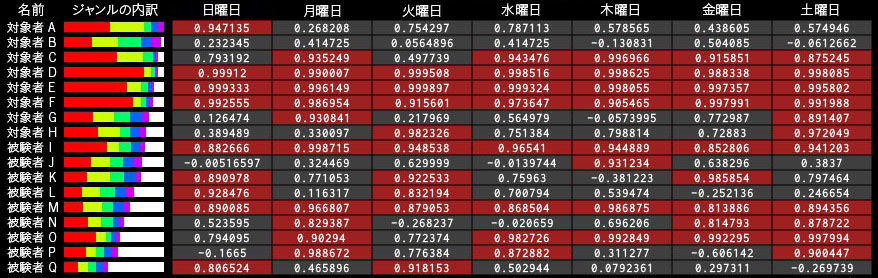
\includegraphics[width = 14cm]{corTable.jpg}
\caption{曜日毎に再生されたものと、音楽ライブラリのジャンルの相関一覧}
\label{corTable}
\end{center}
\end{figure}


\section{考察}
音楽の聴き方は、個人によって、ばらばらであるため、
音楽推薦システムにおいては、
第一にどのような音楽推薦システムがユーザーにとって適しているかを判断するのが重要だと考えられる。

実験の結果から、以下の条件にあてはまる人は、時刻によって音楽を推薦することができないと考えられる。
\paragraph{音楽をあまり聴かない人}
音楽の再生履歴データが少なく、時刻による推薦ができない。
楽曲の数が少ないことが多く、時刻によって再生する音楽を分けることが難しい。

\paragraph{生活が不規則な人}
生活が不規則な人は、曜日や、時刻によって、音楽の聴き方に周期が見られないため、
時刻による推薦は不可能である。

\paragraph{シャッフル再生を常に利用する人}
時刻によって、音楽の選択が変化しないため、
どの時刻にどんな曲を聴きたいのかを推測することができない。
音楽再生のジャンルの内訳が、曜日や時刻によって常に音楽ライブラリ全体と相関が高い場合、シャッフル機能を常に利用していると考えられる。

\paragraph{聴くジャンルが1つに偏っている人}
聴いているジャンルが、1つに偏っている人は、そのジャンルのなかで、シャッフル機能を利用して再生することで十分であると考えられる。

%無理矢理改行
\vspace{\Cvs} 
\par
逆に、以下の条件にあてはまる人は、時刻によって音楽を推薦が可能だと考えられる。
\paragraph{履歴データによる音楽再生のジャンルの内訳が、曜日によって変化する場合}
シャッフル機能による再生をするのではなく、
自分で積極的に選択しているものと考えられる。こういったユーザーへは、
曜日と時刻から推測される楽曲を推薦することで、
普段聴いているような音楽を再生することができると考えられる。
こういったユーザーは、音楽ライブラリ全体のジャンルの内訳と、曜日毎に再生された音楽のジャンルの内訳の相関が小さい。
\paragraph{規則正しく生活している人}
規則正しく生活をしている人は、時刻によってどのような状況にユーザーがいるかが決まっているので、
音楽を再生する時刻と同じ時刻の再生履歴を参照することで、状況にあわせた音楽を再生することができると考えられる。

%無理矢理改行
\vspace{\Cvs} 
また、時刻によって音楽を推薦することができないと考えられる人に対しても、以下の条件がある場合、音楽を時刻で推薦することがよい場合がある。

\paragraph{音楽再生ソフトがスキップしたことを履歴として残す場合}
シャッフル機能を利用している場合であっても、ユーザーが操作を行い、選ばれた楽曲をスキップすることがある。
この操作は、「今はその楽曲を聴きたくない」というユーザーによる意志表示であるので、
シャッフル機能であっても、スキップされた楽曲とその時刻を調べることにより、時刻によるユーザーの好みがわかる可能性がある。

\paragraph{規則正しい時間帯または音楽をいつもかける時間帯をユーザーから取得する}
本実験では、睡眠時間が不規則な人であっても、仕事や授業や移動などは、規則正しく同じ時刻に行われており、
個人の中でも不規則的な生活をする時間と、規則的な生活をする時間があると考えられる。
また、普段の生活の項目の中で、作業中に音楽を聴くと回答した項目は、自分だけの活動でありながら、
アンケートで書かれたことと、音楽の履歴情報が合致していることが多かった。
作業中に関しては、作業がはかどるように音楽を再生するといった、音楽と作業がセットにすることが習慣化しているからだと考えられる。
このため、規則正しい時間、または音楽をいつもかける時間帯をユーザーから取得することで、
ユーザーを``不規則な生活をする人''というマクロな定義で、一気に時刻による音楽の推薦に不適当なユーザーにしてしまうのではなく、
一週間のなかで1つの曜日だけであったり、ある時間帯だけでも一時的に時刻による音楽の推薦が可能になる。

%無理矢理改行
\vspace{\Cvs} 
また、音楽を時刻によって推薦するシステムは、以下のことが実現した場合、
ユーザーの聴きたい音楽を推薦する精度を向上させることができると考えられる。
\paragraph{曜日の切れ目をユーザーに定義してもらう}
曜日の切れ目は、アンケートを参照しなければ分からないことが多いため、
ユーザー自身に設定してもらうことで、
深夜、早朝どちら側の音楽を推薦すべきかを正しく判断して楽曲を推薦することが出来る。

\paragraph{楽曲全てについてジャンル名をユーザーに付けてもらう}
被験者にインタビューする際、具体的に被験者が多く聴くジャンル名を挙げても、
被験者自身がそのジャンルを聴いているという自覚がない場合や、異なるジャンルとして認識している場合があった。
そこで、ジャンル付けをユーザー自身が行うことで、ジャンル名を利用した音楽推薦システムが、
ユーザーが聴きたい音楽を推薦する精度が上がるものと考えられる。
また、被験者にとって、区別がつかないジャンルや、つけていないジャンルがあったり、
サウンドトラックと、sound trackといった、日本語表記と英語表記で2種類のものがあったりしたが、
ユーザーによって、ジャンル分けを行うことによって、1つのジャンルに含まれる楽曲の数が増えることで、
同じ再生履歴の数自体が変わらなくても、1つのジャンルが持つ履歴情報が増えるため、
ジャンルを利用した音楽推薦システムが、ユーザーが聴きたい音楽を推薦する精度が上がるものと考えられる。
\paragraph{楽曲の再生された時刻の履歴が全て残す}
iTunesの仕様により、1つの楽曲に関して、その曲が複数回再生されてた場合でも、
最後に聴いた時刻しか保存されていないが、
楽曲の再生された時刻の履歴をすべて残すことで、
より多くの履歴データを利用できるため、
ユーザーが聴きたい音楽を推薦する精度が高まると考えられる。
また、たくさん聴かれている曲は、よりユーザーが聴きたい楽曲であると推測できるため、
例えば同じ時刻に再生された2つの楽曲があった場合、
1回しか再生されていないものと、
10回その時刻に聴かれたものであったら、10回再生された方を優先して再生することで、
ユーザーが普段聴いている音楽を推薦する精度が向上する。

%\paragraph{音楽再生ソフトが検索履歴を履歴として残す場合}
%シャッフル機能を利用している場合であっても、ユーザーが聴きたい音楽を検索することから


\section{結論}
音楽の聴き方は個人で大きく異なっているが、
個人の中では、その人独自の聴き方があり、
人によって、適切な推薦システムは異なっていることがわかった。
%シャッフル機能について
シャッフル機能を使用した再生が人気なのは、ユーザーの状況や、好みによって、その効果が変化しない点にある。
しかし、それは最大公約数的な良さであって、最適なものだとはいえない。
シャッフル機能よりも、時刻によって音楽を推薦する方が、ユーザーのいつもの音楽再生に沿ったものを推薦できる場合もある。
よって、
ユーザーの音楽ライブラリの内容と、
ユーザーの音楽再生の状況により、
音楽の推薦方式を、
シャッフル、
ジャンルによる推薦、
時刻による推薦の
どれが好ましいかを動的に決定して推薦することによって
ユーザーが再生したい曲を、推薦することができる。

\subsection{今後の展望}
普段自分が選んでいるような音楽を、
自動的に再生することが、音楽推薦の最終形であるとは限らない。
シャッフル機能が人気なのは、無作為で選ばれたものであるのにかかわらず、
絶妙なタイミングで再生されたかのようなときめきを偶然に得るからである。
音楽再生をいつも通りに自動的に再生することによって、単調になるあまり、つまらない再生になる可能性があるため、
あえて、普段聴かない音楽を一部はさむことがよいと推測される。
音楽推薦システムで、普段聴くものに対して、どのくらい普段聴かないものをはさめば、
ユーザーを飽きさせることなく、楽しませることができるのか、今後の課題としたい。

\section{備考}
研究資料および、プログラムの一部は、(個人情報は含まない)
http://yutatoga.com/thesisからダウンロードできる。

\section{参考文献}
\begin{thebibliography}{99}
\bibitem{musicovery}
Musicovery
\par
http://musicovery.com/
\par
最終アクセス日 2012年12月12日
\bibitem{walkman}
WALKMAN
\par
http://www.sony.jp/walkman/
\par
最終アクセス日 2012年12月12日
\bibitem{ipod}
iPod
\par
http://www.apple.com/ipod/
\par
最終アクセス日 2012年12月12日
\bibitem{iPhone}
iPhone
\par
http://www.apple.com/iphone/
\par
最終アクセス日 2012年12月12日
\bibitem{iTunes}
iTunes
\par
http://www.apple.com/itunes/
\par
最終アクセス日 2012年12月12日
\bibitem{oto}
OtO
\par
http://yutatoga.com/oto.html
\par
最終アクセス日 2012年12月12日
\bibitem{musicEarth}
Music Earth
\par
http://yutatoga.com/musicearth.html
\par
最終アクセス日 2012年12月12日

\bibitem{Musicream}
後藤 孝行, 後藤 真孝: Musicream: 楽曲を流してくっつけて並べることので
きる新たな音楽再生インタフェース, WISS2004, pp.53–58 (2004).
%Floyed, E,Toole. ``Loudspeakers and Rooms for Sound Reproduction- A Scientific Review." 
%\bibitem{hogehoge2}
%Floyed, E,Toole. ``Loudspeakers and Rooms for Sound Reproduction- A Scientific Review." 
\end{thebibliography}

\end{document}